\documentclass[../main.tex]{subfiles} % 需要pdf封面

\begin{document}

% STC89xx series, which is produced by STC MCU Limited, is a 8-bit single-chip microcontroller with a fully
% compatible instruction set with industrial-standard 80C51 series microcontroller. There is 64K bytes flash
% memory embeded for appliaction program, which is shared with In-System-Programming code.In-SystemProgramming (ISP) and In-Application-Programming (IAP) support the users to upgrade the program and data
% in system. ISP allows the user to download new code without removing the microcontroller from the actual end
% product;IAP means that the device can write non-valatile data in Flash memory while the application program
% is running. There are 1280 bytes or 512 bytes on-chip RAM embedded that provides requirement from wide
% field application. The user can configure the device to run in 12 clocks per machine cycle, and to get the same
% performance just as he uses another standard 80C51 device that is provided by other vendor, or 6 clocks per
% machine cycle to achieve twice performance. The STC89xx series retain all features of the standard 80C51. In
% addition, the STC89xx series have a extra I/O port (P4 ), Timer 2, a 8-sources, 4-priority-level interrupt structure,
% on-chip crystal oscillator,and a one-time enabled Watchdog Timer.
\subsubsection{STC89系列芯片}

  STC89系列是8位单片机,
  有$\SI{64}{KiB}$flash 存储空间,
  $\SI{512}{B}$或$\SI{1080}{B}$的RAM存储空间,
  此外该系列有额外的I/O端口$P_4$,
  时钟$T_2$,
  4个优先级的中断系统

\subsubsection{开发版部件}
  该开发版部件示意图如%
  \cref{fig:board}
  
  \begin{figure}[H]
    \centering
    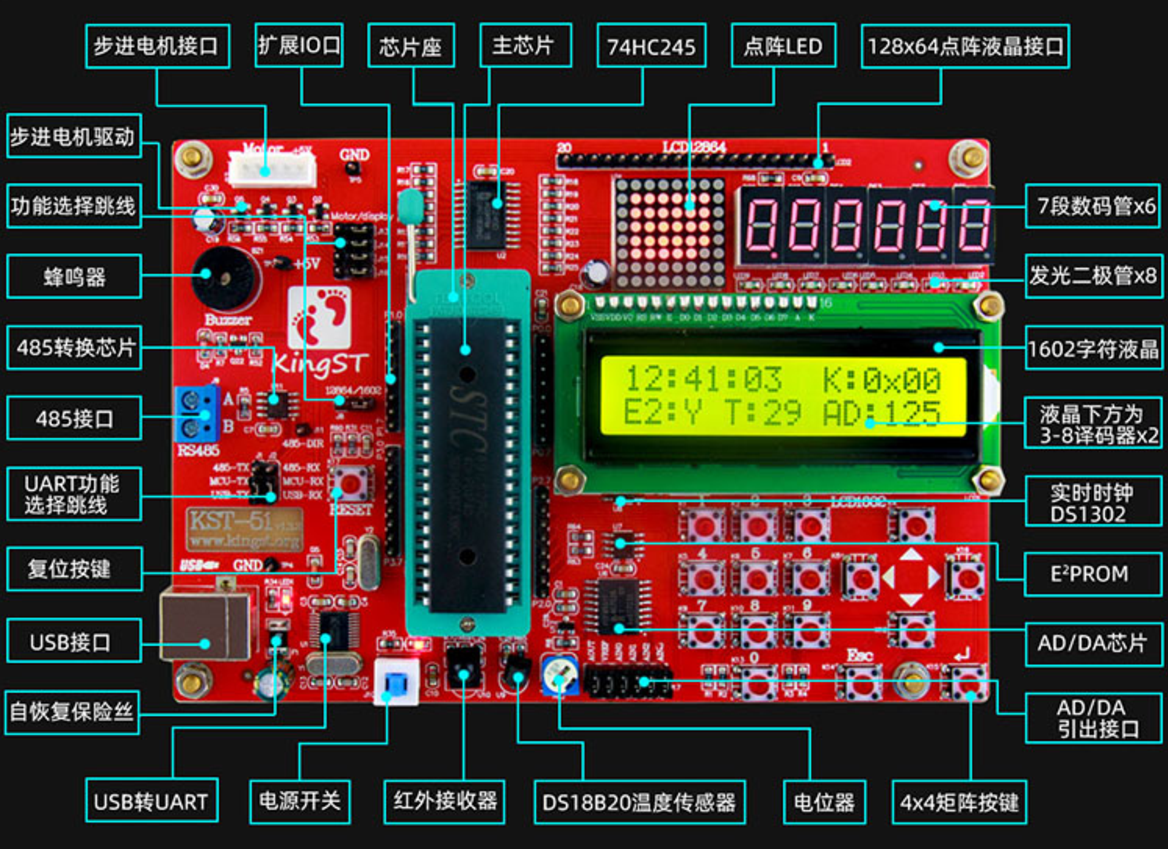
\includegraphics[width = 0.8\textwidth]{board}
    %\missingfigure{board}
    \caption{开发版资源示意图\upcite{files}}
    \label{fig:board}
  \end{figure}
  本项目主要使用$4 \times 4$矩阵按键,7段数码管,
  点阵LED,反光二极管作为相关功能的实现和展示



\end{document}
